\section{Stochastic Gradient Descent (SGD)}
\frame{\tableofcontents[currentsection, hideothersubsections]}

\begin{frame}
\frametitle{SGD: Intro}

WHAT:\\
Stochastic Gradient Descent (SGD);
\vspace{5mm}

WHY:\\
do not know $D$, so do not know the gradient of $L_D(w)$.
\vspace{5mm}

HOW:\\
take a step along a random direction (vector), as long as
its expected value at each iteration will equal the gradient direction
(more generally, a subgradient of the function at the current vector)
\end{frame}

\begin{frame}
\frametitle{SGD: Intro}

\begin{figure}
    \centering
    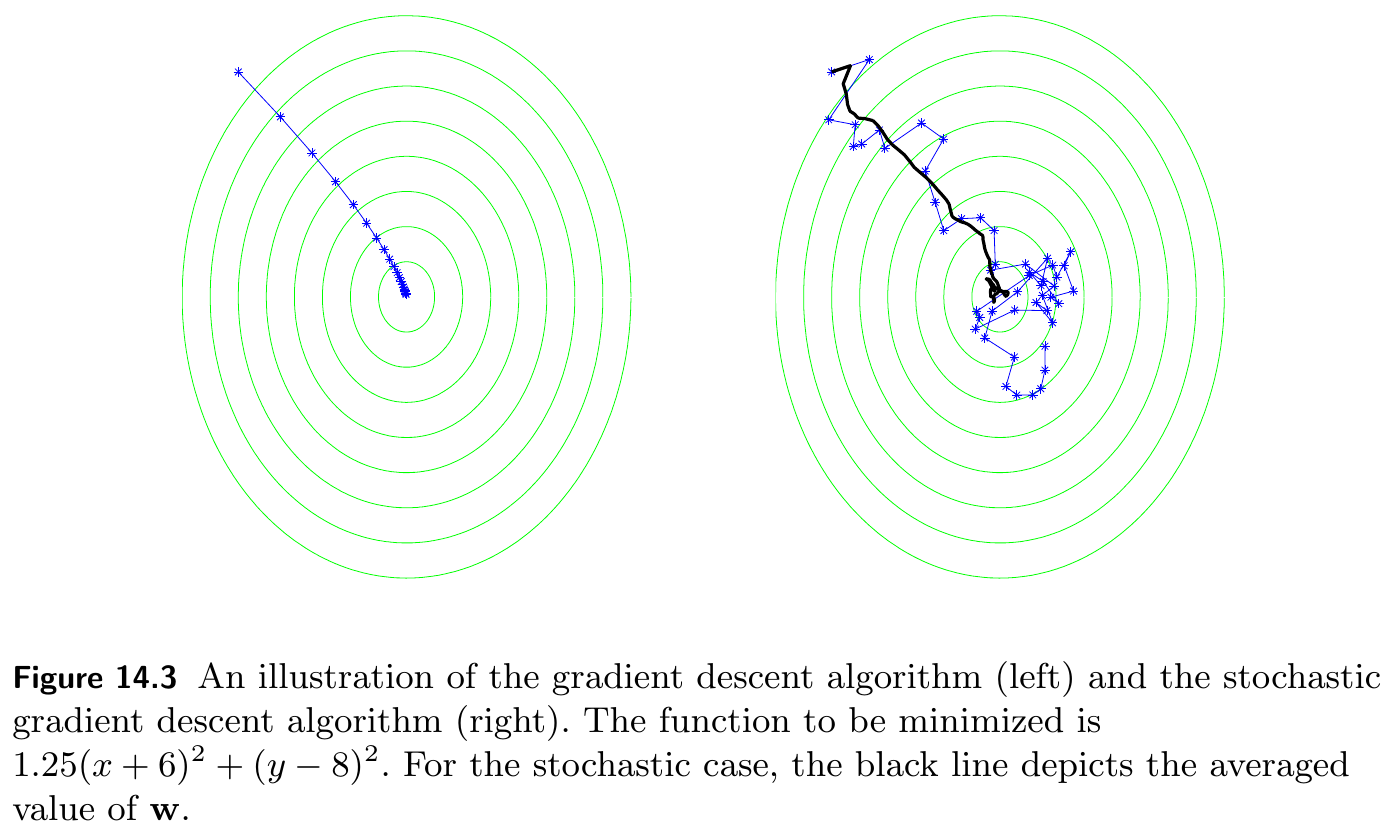
\includegraphics[scale=0.3]{fig_14_3}
\end{figure}

\end{frame}

\begin{frame}
\frametitle{SGD: Intro}

\begin{figure}
    \centering
    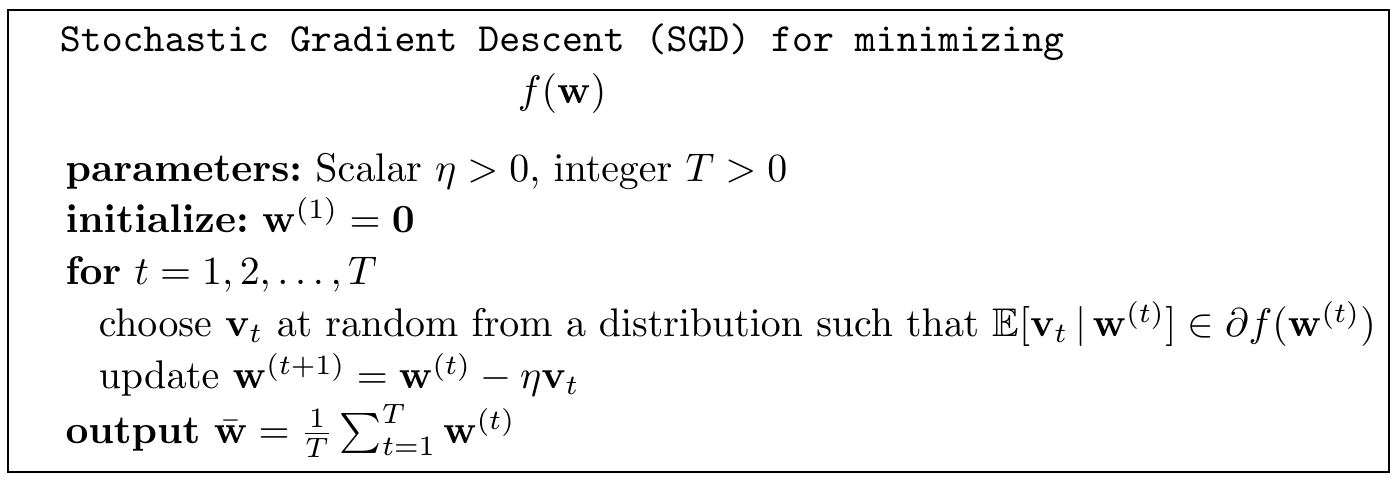
\includegraphics[scale=0.325]{sgd}
\end{figure}

\end{frame}



\begin{frame}
\frametitle{SGD: Analysis for Convex-Lipschitz-Bounded Fn}

\begin{figure}
    \centering
    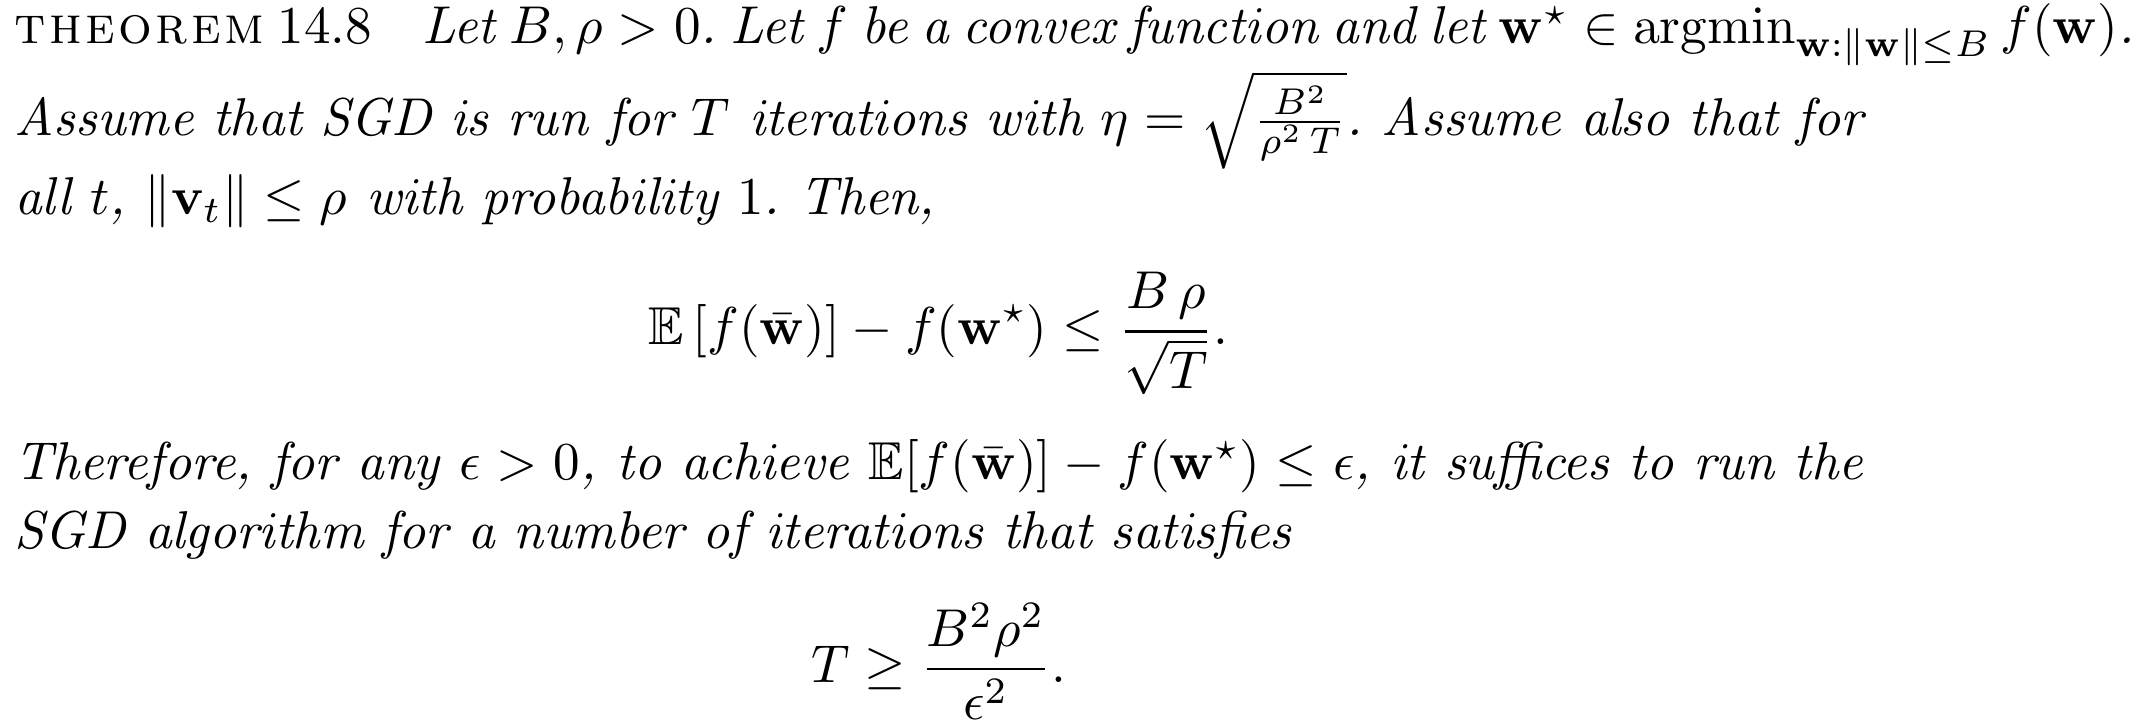
\includegraphics[scale=0.2]{theorem_14_8}
\end{figure}

\end{frame}
